\documentclass[10pt]{article} % 10, 11,12 allowed only
\usepackage[T1]{fontenc}
\usepackage{lipsum}
\usepackage{graphicx}
\usepackage{amsmath}


\title{Hello Saklain}
\author{Saklain Hasan}
\date{June 2026}
\begin{document}

\maketitle

\tableofcontents

\section{Introduction}

\lipsum[1-6]

\subsection{Intro I}
\lipsum[5-7]

\subsubsection{Intro II}
\lipsum[8]

\subsubsection{Intro III}
\lipsum[9]

\subsubsection*{Intro IV}          % * dile oita te numbering hobe na
\lipsum[8]

\subsubsection{Into V}
\lipsum[9]

\paragraph{What is NP-Complete?} \lipsum[9]
\subparagraph{Tintin} \lipsum[4]

\section{List}

listing here we go:


Ordered
\begin{enumerate}
    \item An entry
    \item Another one
    \item Wow! three entries
\end{enumerate}

Unordered
\begin{itemize}
    \item An entry
    \item Another one
    \item wow 3 number entry
\end{itemize}

Description
\begin{description}
    \item[Tintin] Hehe tintin shera
    \item[Doraemon] Doraemon ekti bhodro biral
    \item[Tuba] Tuba ekti gadha baccha   
\end{description}



\begin{enumerate}
    \item An entry
    \item Another one \begin{enumerate}
        \item this is allowed
        \item this is baccha
    \end{enumerate}
    \item Wow! three entries
\end{enumerate}





\section{Saklain er paglami}
Hey world! What is happeining here.

I am Saklain.

tintin


This is a simple document\footnote{with a footnote}

\{ \}        \$ \% \# \& \_  \textbackslash \textasciicircum \textasciitilde \textasciimacron 


Some text with \emph{emphasis and \emph{nested} content} %emphasis er bhitore emphasis dile oita normal hoye jay

Some text in \textit{italic and \textit{nested} content} %italic er bhitoreo italic ee thakbe

Some text in \textbf{boldface and \textit{nested} content}

{\tiny Bangladesh will someday win XYZ world cup!}

{\small Bangladesh will someday win XYZ world cup!}

{\large Bangladesh will someday win XYZ world cup!}

{\Large Bangladesh will someday win XYZ world cup!}

{\LARGE Bangladesh will someday win XYZ world cup!}

%{\huge Bangladesh will someday win XYZ world cup!}

%{\Huge Bangladesh will someday win XYZ world cup!}

% duibar newline dilei khali main pdf e newline hoy ... ekbar newline dile hoyna

\section{Including Graphics}\label{sec_in_graphics}
\begin{figure}[ht]
    \centering
    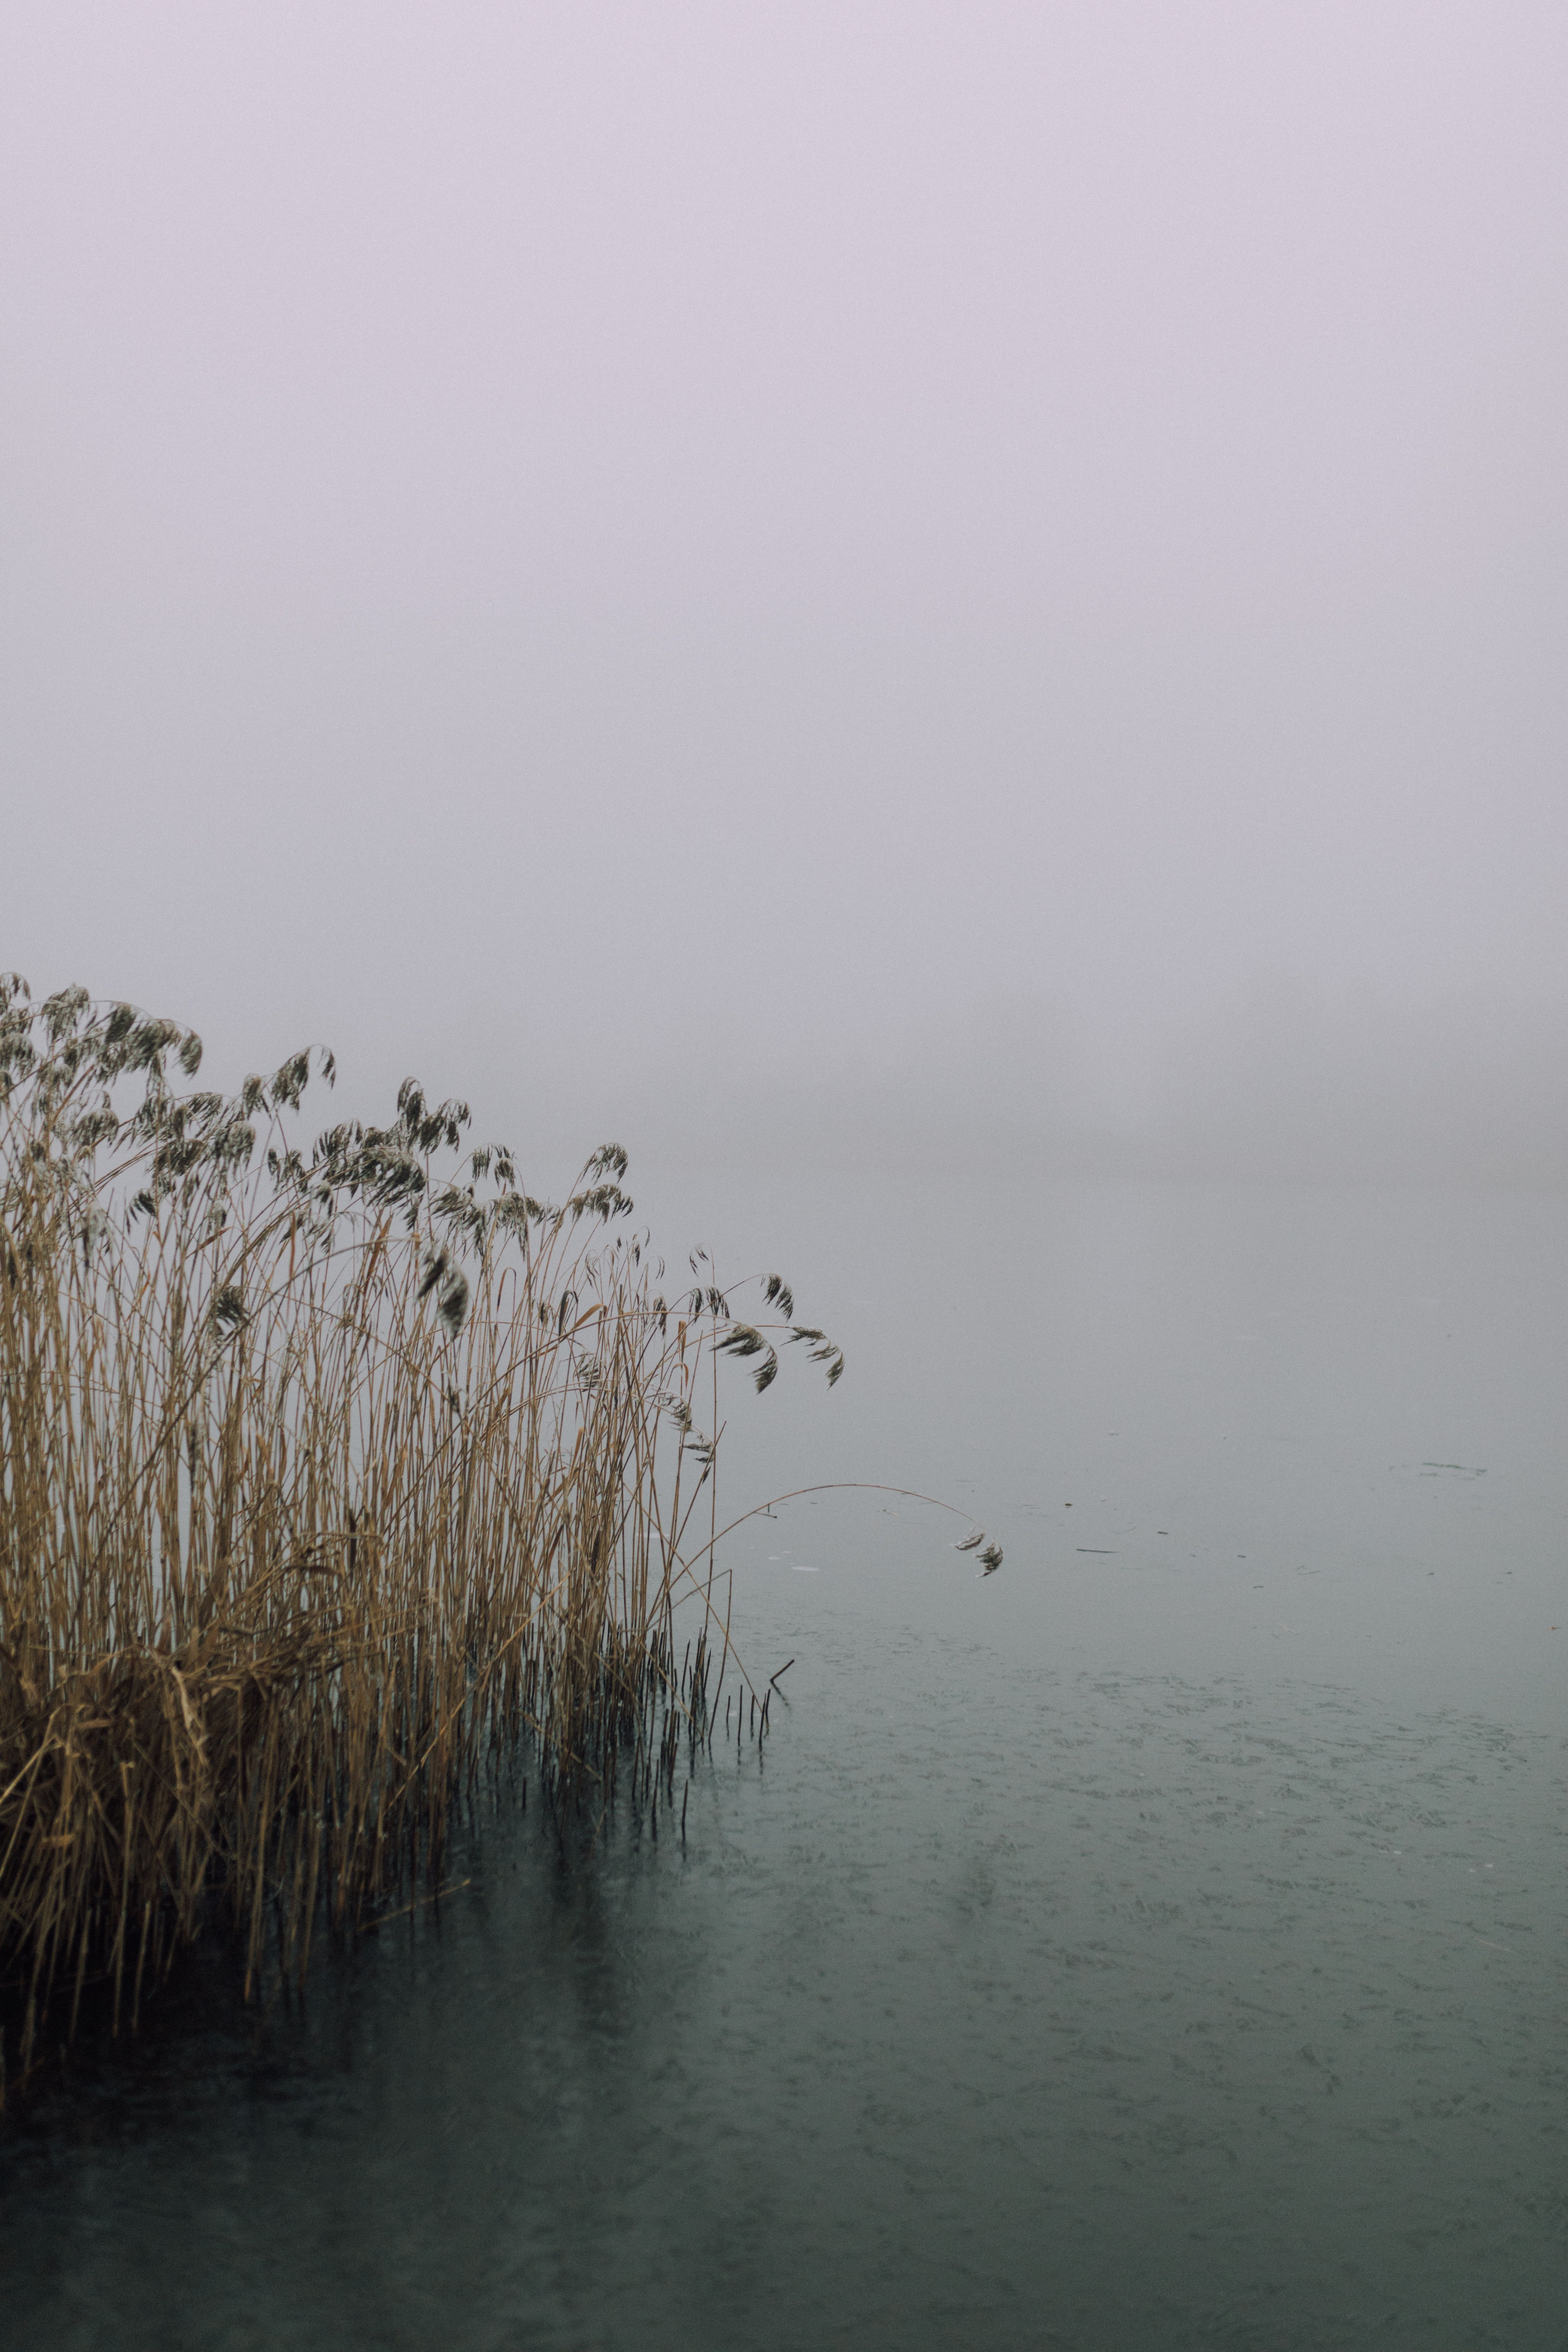
\includegraphics[height=5cm]{fog.jpg}
    \caption{Foggy Lake}
\end{figure}

\begin{figure}[ht]
    \centering
    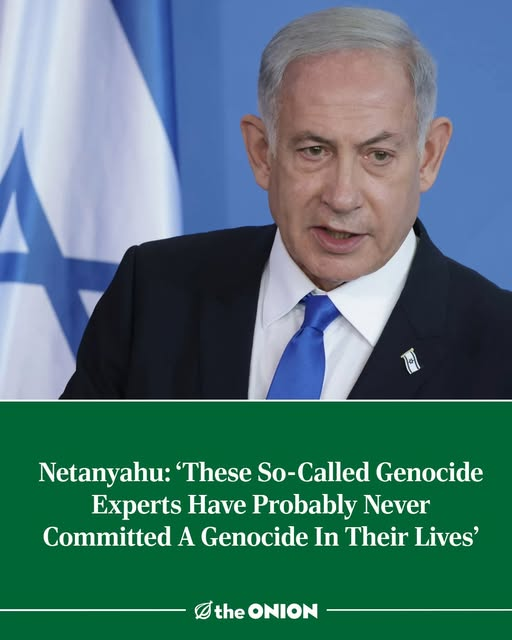
\includegraphics[width=0.5\linewidth]{israel.jpg}
    \caption{Netanyahu being insane for 69th time}
\end{figure}



\begin{figure}[htbp]
    \centering
    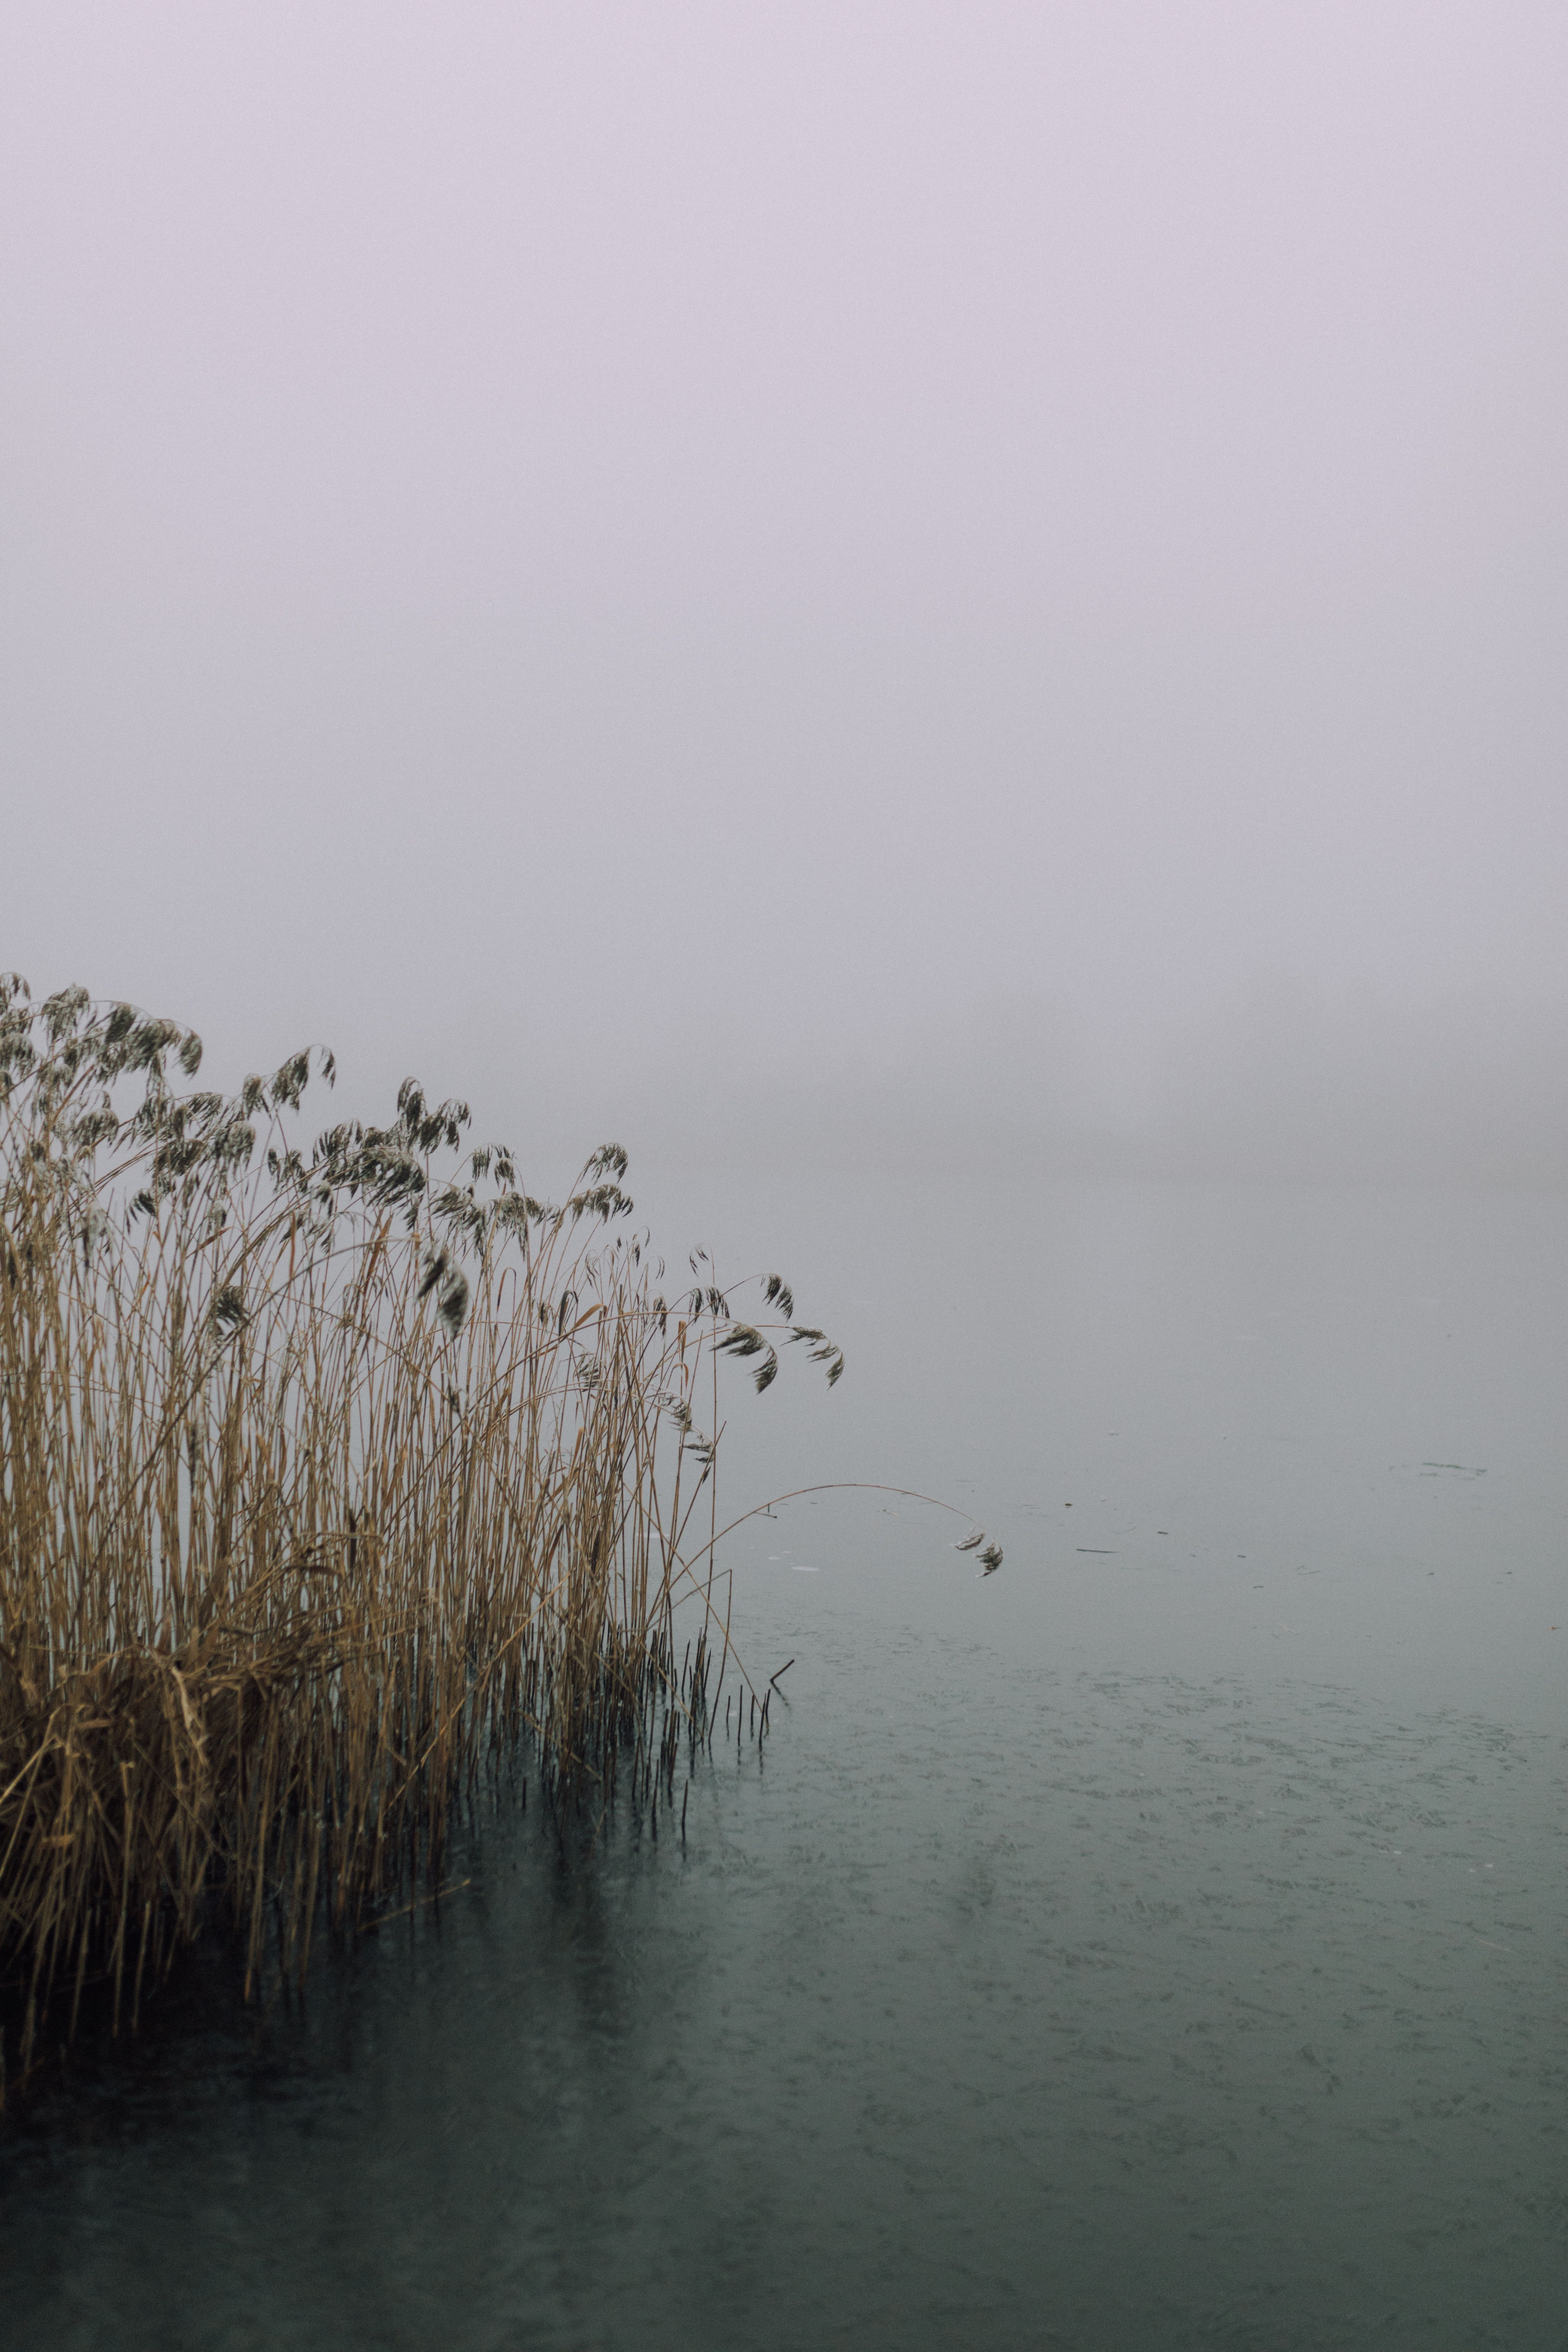
\includegraphics[height=6cm]{fog.jpg} % Shrunk slightly to help it fit
    \caption{Foggy Lake}
    \label{fig:lake}
    
    \vspace{0.5cm} % Adjusts the gap between the two images manually
    
    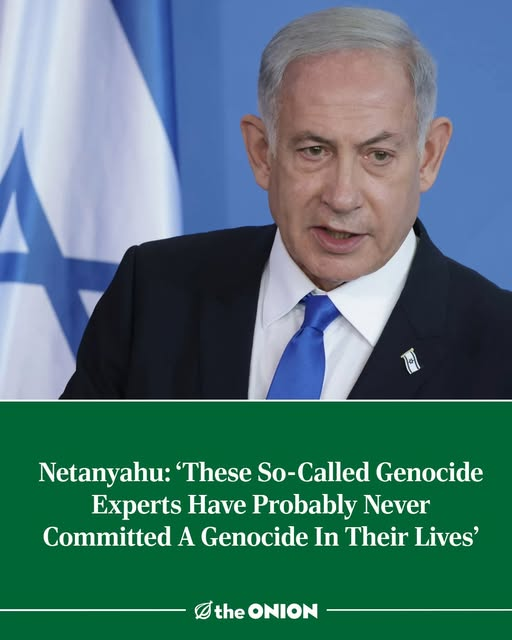
\includegraphics[width=0.5\linewidth]{israel.jpg}
    \caption{Netanyahu being insane for 69th time}
    \label{fig:devil}
\end{figure}

\clearpage

In Figure~\ref{fig:devil}, we can see a person who loves committing genocide.




\section{Alignment}

\textbf{tables are here:}

\vspace{1cm}


\begin{tabular}{|l|l|l|}
    \hline
    Animal & Food & Size \\ \hline
    dog & meat & medium \\ \hline
    horse & hay & large \\ \hline
    frog & flies & small \\ \hline
\end{tabular}

\vspace{1cm}

\begin{tabular}{ccc}
    Animal & Food & Size \\
    dog & meat & medium \\
    horse & hay & large \\
    frog & flies & small \\
\end{tabular}

\vspace{1cm}


\begin{tabular}{rrr}
    Animal & Food & Size \\
    dog & meat & medium \\
    horse & hay & large \\
    frog & flies & small \\
\end{tabular}



\newpage

\section{Mathematics}
We want to write the solution for the quadratic equation $$ax^2 +bx+c=0$$

The solution is 
$$
 x= \frac{-b \pm \sqrt{b^2-4\cdot a\cdot c}}{2a}
$$

\end{document}